\newpage
\section{LECTURE 4}

\section{Agenda}
This lecture covers constrained minimization.

\section{Equality Constraints}
Let's consider the following minimization problem, subject to some \textit{equality constraints}: 
\begin{align}
    \min_x f(x) \ \ &; \ \ f(x) : \mathbb{R}^n \longrightarrow \mathbb{R} \\
    \ni c(x) = 0 \ \ &; \ \ c(x) :  \mathbb{R}^n \longrightarrow \mathbb{R}^m
\end{align}

\subsection{First order necessary conditions}
The first order necessary conditions for the $x$ at which the function attains its minimum:
\begin{itemize}
    \item Need $\nabla f(x) = 0$ in the unconstrained / free directions. 
    \item Need $c(x)=0$
\end{itemize}

\begin{figure}
    \centering
    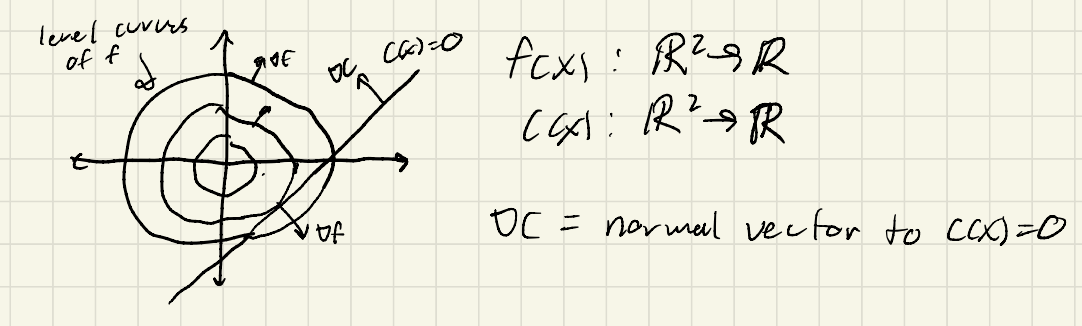
\includegraphics[width=0.4\linewidth]{L4_Images/EqC.PNG}
    \caption{Level curves of $f(x)$}
    \label{fig:l4f1}
\end{figure}

\noindent
Thus any non-zero component of $\nabla f$ must be normal to the constraint surface / manifold. 
\begin{align}
    \nabla f + \lambda \nabla c = 0 \ \textrm{for some} \ \lambda \in \mathbb{R}
\end{align}
where $\lambda$ is a Lagrange multiplier or ``Dual variable''. In general, we have that:
\begin{align}
    \frac{\partial f}{\partial x} + \lambda^T \frac{\partial c}{\partial x} = 0
\end{align}
Based on this gradient condition, we define: 
\begin{align}
    L(x,\lambda) = f(x) + \lambda^T c(x)
\end{align}
where $L(x, \lambda)$ represents the Lagrangian. This is subject to: 
\begin{align}
    \nabla_x L(x,\lambda) &= \nabla f + (\frac{\partial c}{\partial x})^T \lambda = 0 \\
    \nabla_{\lambda} L(x,\lambda) &= c(x)
\end{align}
Together, these conditions represent the KKT conditions. We can now solve this jointly in $x$ and $\lambda$ as a root finding problem, using Newton's method. 
\begin{align}
    \nabla_x L (x + \Delta x, \lambda + \Delta \lambda) &\approx \nabla_x L (x, \lambda) + \frac{\partial^2 L}{\partial x^2} \Delta x + \frac{\partial^2 L}{\partial x \partial \lambda} \Delta \lambda  \\
    \nabla_{\lambda} L (x + \Delta x, \lambda) &\approx c(x) + \frac{\partial c}{\partial x} \Delta x
\end{align}
where $\frac{\partial^2 L}{\partial x \partial \lambda} = (\frac{\partial c}{\partial x})^T$. 
This can be written as the following matrix system:
\begin{align}
    \begin{bmatrix}
        \frac{\partial^2 L}{\partial x^2}  &  (\frac{\partial c}{\partial x})^T \\
        \frac{\partial c}{\partial x} & 0 
    \end{bmatrix}
    \begin{bmatrix}
        \Delta x \\
        \Delta \lambda
    \end{bmatrix}
    = 
    \begin{bmatrix}
        -\nabla_x L(x,\lambda) \\
        - c(x)
    \end{bmatrix}
\end{align}
The first matrix here is the Hessian of the Lagrangian, and describes the KKT system. 

\subsection{Gauss-Newton Method}
\begin{align}
    \frac{\partial^2 L}{\partial x^2} = \nabla^2 f + \frac{\partial}{\partial x} \big[ (\frac{\partial c}{\partial x})^T \lambda \big]
\end{align}
Here, $\frac{\partial}{\partial x} \big[ (\frac{\partial c}{\partial x})^T \lambda \big]$ is expensive to compute. We often drop this term, ignoring the ``constraint curvature''. 
Dropping this term is called Gauss-Newton method. This is equivalent to linearizing the system first, and then performing Newton's method. 

\noindent
Check out the example from the Lecture on this. 

\subsection{Take-Away Message}
\begin{itemize}
    \item May need to regularize $\frac{\partial^2 L}{\partial x^2}$ in Newton's method, even if $\nabla^2 f=0$. 
    \item Gauss-Newton is often used in practice because it converges almost as fast, and is cheaper per iteration. 
\end{itemize}

\section{Inequality constraints}
More generally, we have to reconcile with inequality constraints as well. Consider a minimization problem subject to inequality constraint: 
\begin{align}
    \min_x f(x) \\
    \ni c(x) \geq 0
\end{align}
Let's look at the case of purely inequality constraints for now. In general, these methods are combined with the equality constraint methods above, to handle general inequality / equality constraints  in the same problem. 

\subsection{First-Order Necessary Conditions}
As before, the first order conditions specify that - 
\begin{itemize}
    \item Need $\nabla f(x) = 0$ in the unconstrained / free directions. 
    \item Need $c(x) \geq 0$ \ \ \textrm{Note the inequality here.}
\end{itemize}
Mathematically, 
\begin{align}
    \nabla f - (\frac{\partial c}{\partial x})^T \lambda &= 0 \gets \textrm{"Stationarity"} \\
    c(x) &\geq 0 \gets \textrm{"Primal Feasibility"}
    \lambda &\geq 0 \gets \textrm{"Dual Feasibility"}
    \lambda^T c(x) &= 0 \gets \textrm{"Complementarity"}
\end{align}
Together, these conditions specify the full set of KKT conditions. 

\subsection{Intuition}
The intuition for these conditions is as follows: 
\begin{itemize}
    \item If constraint is active, (we are on the constraint manifold), we have $c(x) = 0 \implies \lambda = 0$. This is the same as the equality case. 
    \item If the constraint is inactive, we have $c(x)>0 \implies \lambda = 0$, which is the same as the \textit{unconstrained} case. 
    \item Essentially complementarity ensures either one of $\lambda$ and $c(x)$ will be $0$, or ``on /off switching'' of constraints.
\end{itemize}

\subsection{Algorithms}
The implementation of optimization methods here is much hard than the equality case; we can't directly apply Newton's method to the KKT conditions. There are many options we can use, with different trade offs. 

\subsection{Active-Set Method}
\begin{itemize}
    \item Applies when you have a good way of knowing which constraints are active / inactive.
    \item Solves equality constrained problem (when it is active). 
    \item Very fast if you have a good heuristic. 
    \item Can be very (combinatorially) bad if you don't know which constraints are active. 
\end{itemize}

\subsection{Barrier / Interior-Point Method}
\begin{itemize}
    \item We replace the inequalities with a ``barrier function'', in the objective, that blows up at the constraint boundary \cref{fig:l4f2}.
    \item This is the gold standard for small to medium \textit{convex} problems.
    \item Requires a lot of hacks and tricks to get working for non-convex problems.
\end{itemize}
\begin{figure}
    \centering
    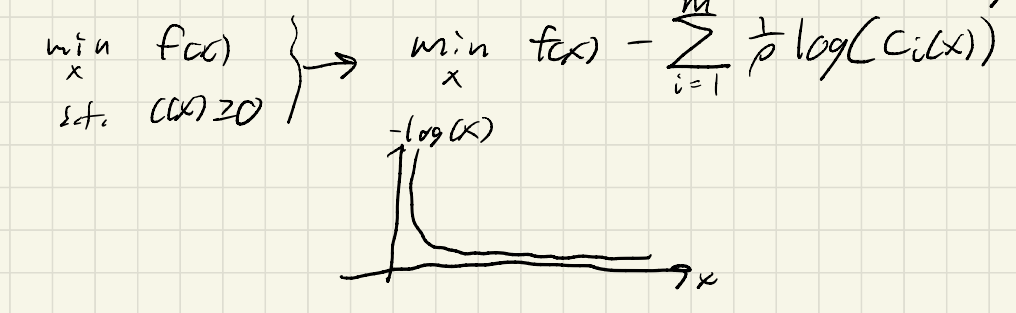
\includegraphics[width=0.4\linewidth]{L4_Images/I2.PNG}
    \caption{Barrier Function}
    \label{fig:l4f2}
\end{figure}

\subsection{Penalty Method}
\begin{itemize}
    \item Replace the inequality constraint with an objective term that penalizes violations \cref{fig:l4f3}.
    \item It's easy to implement. 
    \item Has issues with being ill-conditioned (the Hessian has a huge spread of eigenvalues, that causes Newton's method to struggle). 
    \item Difficult to achieve high accuracy.
\end{itemize}
\begin{figure}
    \centering
    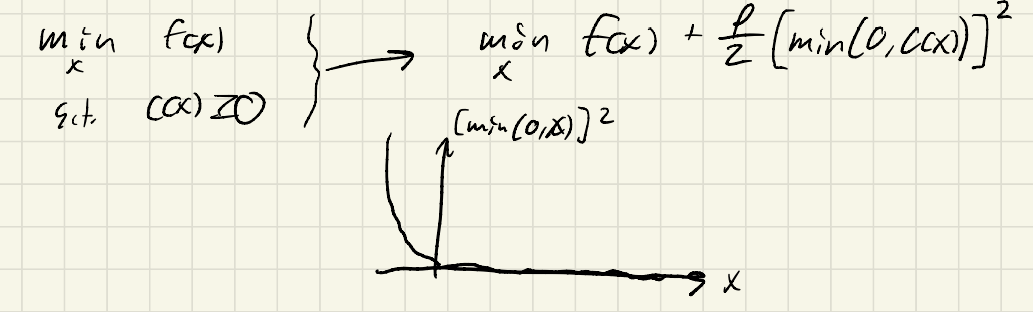
\includegraphics[width=0.4\linewidth]{L4_Images/I3.PNG}
    \caption{Penalty Method Objective}
    \label{fig:l4f3}
\end{figure}

\subsection{Augmented Lagrangian}
\begin{itemize}
    \item Add a Lagrange multiplier estimate to the penalty method,  to fix issues that penalty method faced.
\end{itemize}
\begin{align}
    \min_x f(x) - \tilde{\lambda}^T c(x) + \rho /2 \big[ \min(0,c(x)) \big]^2
\end{align}
where $f(x) - \tilde{\lambda}^T c(x) + \rho /2 \big[ min(0,c(x)) \big]^2 = L_{\rho}(x,\lambda)$ is the augmented lagrangian. 
Remember, here we want to penalize the constraints being violated, that's why we have a $-\tilde{\lambda}$ instead of $+\lambda$.
We first minimize with respect to $x$ (with a fixed $\tilde{\lambda}$, and then we update $\tilde{\lambda}$ by ``offloading'' penalty term at each iteration: 
\begin{align}
    \frac{\partial f}{\partial x} - \tilde{\lambda} \frac{\partial c}{\partial x} + \rho c(x)^T \frac{\partial c}{\partial x} = \frac{\partial f}{\partial x} - \big[ \tilde{\lambda} - \rho c(x) \big]^T \frac{\partial c}{\partial x} = 0
    \implies \tilde{\lambda} \gets \tilde{\lambda} - \rho c(x) \ \textrm{for active constraints}.
\end{align}
Algorithmically, this can be expressed as: 
\\
\\
\noindent
\begin{algorithm}
	\caption{Augmented Lagrangian method}
	\label{alg:auglag}
	\begin{algorithmic}[1]	
	    \While {Not Converged} 
            \State $\min_x L_{\rho} (x, \tilde{\lambda}$ \Comment{Minimize w.r.t $x$.}
            \State $\tilde{\lambda} \gets \tilde{\lambda} - \min(0,\rho c(x)) $ \Comment{Update the multipliers.}
            \State $\rho \gets \alpha \rho$ \Comment{Increase penalty. Typically, $\alpha \approx 10$}
        \EndWhile
	\end{algorithmic}
\end{algorithm}
\\
\\
\begin{itemize}
    \item This fixes the ill-conditioning that penalty method suffers. 
    \item It converges fast (super-linearly) to moderate precision. 
    \item Works well on non-convex problems too! 
\end{itemize}

\subsection{Quadratic Program Example!}
Consider the problem: 
\begin{align}
    \min_x \ \frac{1}{2} x^T Q x &+ q^T x \ \ \ni Q >0  \ \textrm{(Convex)} \\
    \ni Ax &\leq b \\
    \ni Cx &= d
\end{align}
Here have a quadratic objective, and linear constraints. This type of problem is very common and useful in control, and can be solved very fast online (in the order of KHz).
Remember to check out the example in the lecture video! 

\subsection{Additional Notes}
\begin{itemize}
    \item In general, we still need regularization and line searches in the constrained setting. 
    \item Linear searches get a little more complicated. 
\end{itemize}

\section{References}
Remember to check out \cite{nocedal2006numerical} for more on constrained minimization! 

\printbibliography